\section{Introduction}\label{SecIntro}

\marginnote{MH: I don't really like first sentence}
With the emergence of a new generation of trusted personal devices
(mobile phones, PDAs, smart cards \emph{etc.}), the demand for
techniques to ensure the security of applications has become even more
prominent. A common way to ensure the security of an application is to
monitor its execution with a security automaton~\cite{Schneider99}.
Upon entry or exit of a security-critical method, the security
automaton changes its internal state. If it reaches an ``illegal''
state, the application will be stopped and a security violation will
be reported. This approach is in particular suited to monitor
properties that are expressed as sequences of legal method calls, such
as life cycle properties, or constraints that express how often or
under which conditions a method can be called.

However, for many applications, such a runtime monitoring approach is
not suited. In particular, if an application is installed on a
stand-alone personal device that is handed out to an end-user, it is
unacceptable that the device could be suddenly blocked, because of a
security violation, and that the end-user would have to return to the
provider to unblock the device.  Instead, for such applications
statical means to enforce security are necessary. A commonly advocated
approach is to require that the application carries a correctness
proof with it, which can be validated before installing the application
on the device. In such a proof carrying code scenario~\cite{Necula97},
the application provider is required to create this proof. Traditional
proof carrying code has focused on simple security properties that can
be checked with a type checker. Within the
\textsf{Mobius} project (see \texttt{http://mobius.inria.fr}),
a more advanced proof carrying code scenario is developed where
security properties are encoded as logical formulae, and classical
program verification techniques are used to produce the proof.

However, typical program verification tools that can be used in such
an approach use a Hoare logic style for the specifications
(\emph{i.e.}, using pre- and postconditions), while security experts
often characterise security requirements by a collection of security
rules that have to be followed by the application developer. Automata
or temporal logic are a natural and intuitive formalism to express
such security rules. Therefore, as a first step towards static
verification of security properties, this paper proposes a translation
from security properties expressed as an automaton (or a safety
temporal logic formula, which can be translated into an
automaton~\cite{Wolper01}) into inline annotations. Based on these
annotations, appropriate Hoare-style specifications can be generated,
see~\cite{PavlovaBBHL04} for a propagation algorithm that does exactly
this.

Since the Java Virtual Machine (and variations) is the most common
platform for personal devices\footnote{The standard Java set-up for
such devices is the Connected Limited Device Configuration, see
\texttt{http://java.sun.com/products/cldc/}, together with the MIDP
profile, see \texttt{http://java.sun.com/products/midp/}.}, we use JML
as the program verification specification language.  JML (Java
Modeling Language)~\cite{LeavensPCCRCK05} is a behavioural interface
specification language for Java. It allows to express Hoare-style
specifications, including advanced constructs like class invariants
and history constraints. Several tools and techniques exist that allow
to validate JML specifications \emph{w.r.t.}\ a Java implementation,
\emph{e.g.},\ static verification is provided by
for example, ESC/Java~\cite{CokK04} and
JACK~\cite{BartheBCGHMPPSV06}, while runtime checking is possible
using the \texttt{jmlc} and \texttt{jmlrac} tools. The JML runtime
checking tools evaluate at every method entry or exit point
preconditions or postconditions, class invariants, history constraints
\emph{etc.}, and if an annotation is violated, an exception is
returned. In addition, at any point in the program code, an assertion
can be added, that is supposed to hold whenever control reaches this
point.

This paper discusses the first step of the translation: from security
automaton to inline annotations. We prove that our translation is
security preserving: if the application monitored by the automaton
does not produce a security violation, runtime checking of the
generated JML annotations will not produce an annotation
exception. The next step will be to propagate the annotations (as
described in~\cite{PavlovaBBHL04}), which means that the annotations
that are generated directly give rise to new program
annotations. Eventually, this will produce a completely annotated
application, and if it can be proven statically that the annotated
program respects its annotations, it also respects the security
property expressed by the automaton.

The translation described in this paper is defined in several
steps. For each step we provide a correctness proof.
First we define a translation from a partial automaton,
\emph{i.e.},\ an automaton that can get \emph{stuck}, because it has
no transition enabled, to a complete automaton, \emph{i.e},\ an
automaton that always has a transition enabled, but that contains a
special \textsf{halted} state, that models that an error has occurred,
and from which one cannot leave. Often it is much more intuitive to
specify a security property by a partial automaton, because this
avoids that the automaton is cluttered up with transition that
\emph{``go wrong''}. However, for many tools and algorithms, a total
automaton is easier to handle. We show that the behaviour of a program
that is monitored with a partial automaton is equivalent to the
behaviour of a program that is monitored with a complete
automaton. Then we define how the complete monitor gives rise to
annotations. We do this by adding special ghost variables to model the
monitor state. To every method specification, we add special
\textsf{set} annotations that update the ghost variables upon entry
and exit of a method~--~according to the updates in the automaton. To
write  this in a convenient way, we introduce a special
conditional construct to update ghost variables (called
\CaseJML). We show that the run-time monitoring of the program
only throws a (new) exception to signal an annotation violation if the
monitor reaches the \textsf{halted} state. Next, we inline the
\textsf{set} annotations from the method specification to the method
body. This requires a code transformation, to ensure that the ghost
variables are also updated appropriately if the method throws an
exception. We prove that the run-time checking behaviour of the
program with the inlined \textsf{set} annotations is equivalent to the
run-time checking behaviour of the program with the method
specification-level \textsf{set} annotations. Finally, as a last step,
we show that the special \CaseJML construct can be transformed
into a sequence of set instructions, and we prove again that this does
not change the run-time checking behaviour of the program. All results
in the paper have been established formally using the PVS theorem
prover~\cite{OwreRRSS96}. The complete formalisation is available via
\texttt{http://www....}.

% TODO: describe the new version of the example
% MH: not necessary to change, maybe just add one line about distinction
% between entry and exit (but the terminate successfully is sufficient)
% AT: But we should say that reset is not allowed within sendSMS, otherwise we
% could make a simpler automaton with just one state and events for normal
% termination of sendSMS and reset.
Throughout this paper, we will use a simple example property to
illustrate the different translations: the method \texttt{sendSMS} can
be called and terminate successfully at most \(N\) times in between
calls to a \texttt{reset} method (notice that the counter is not
increased upon exceptional termination of
\texttt{sendSMS}). Figure~\ref{FigExample} shows a security automaton
that can be used to monitor this property. Even though very basic,
this example is representative for a wide range of important
resource-related security properties.

\marginnote{psfrag needed to improve layout}

\begin{figure}[t]
\begin{center}
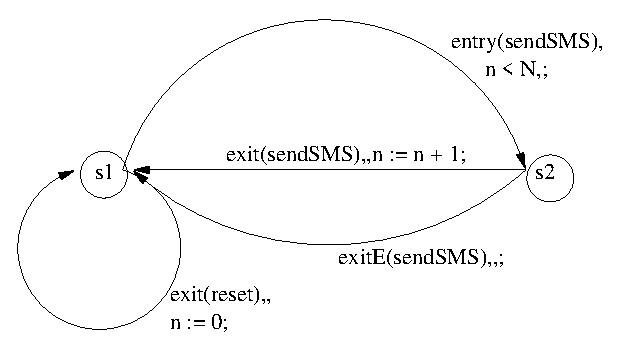
\epsfig{file=limited_sms_alt.eps, width=4cm}
\end{center}
\caption{Example Security Automaton}\label{FigExample}
\end{figure}

The remainder of this paper is organised as
follows. Section~\ref{SecMVA} formalises the automaton format that we
use, and defines completion of an automaton. Next,
Section~\ref{SecProgram} defines the semantics of monitored and
annotated programs. Then Section~\ref{SecAnnotGen} presents the
different translations, and proves their
correctness. Section~\ref{SecRelated} discusses related work, while
Section~\ref{SecConcl} concludes and discusses future work.

